\section{Introduction}\label{sec:intro}
In this chapter, the problem addressed in this Master Thesis is introduced. First, the bridge type and its characteristics are described in Section \ref{sec:int_back}, supplemented by a brief historic integration. In Section \ref{sec:int_prob}, the problem is stated and defined. Ultimately, in Section \ref{sec:int_def}, an orientation about the terminology and the abbreviations is given. 

\subsection{Background}\label{sec:int_back}
Network tied-arch bridges are composed of the arches, the tie girder and the hangers. The tie girder acts as a tension chord tying the arch ends and supporting the horizontal forces. The deck may be integrated into the tie girder (composite deck system) or be supported vertically on deck cross girders (floating deck system). The arches are arranged in planes which can either be vertical or inclined. Each plane usually features two hanger sets, which connect the tie and the arch and cross each other multiple times. The structural components for a floating deck system are illustrated in Fig. \ref{fig:components_illustration}.

\begin{figure}[H]
    \centering
    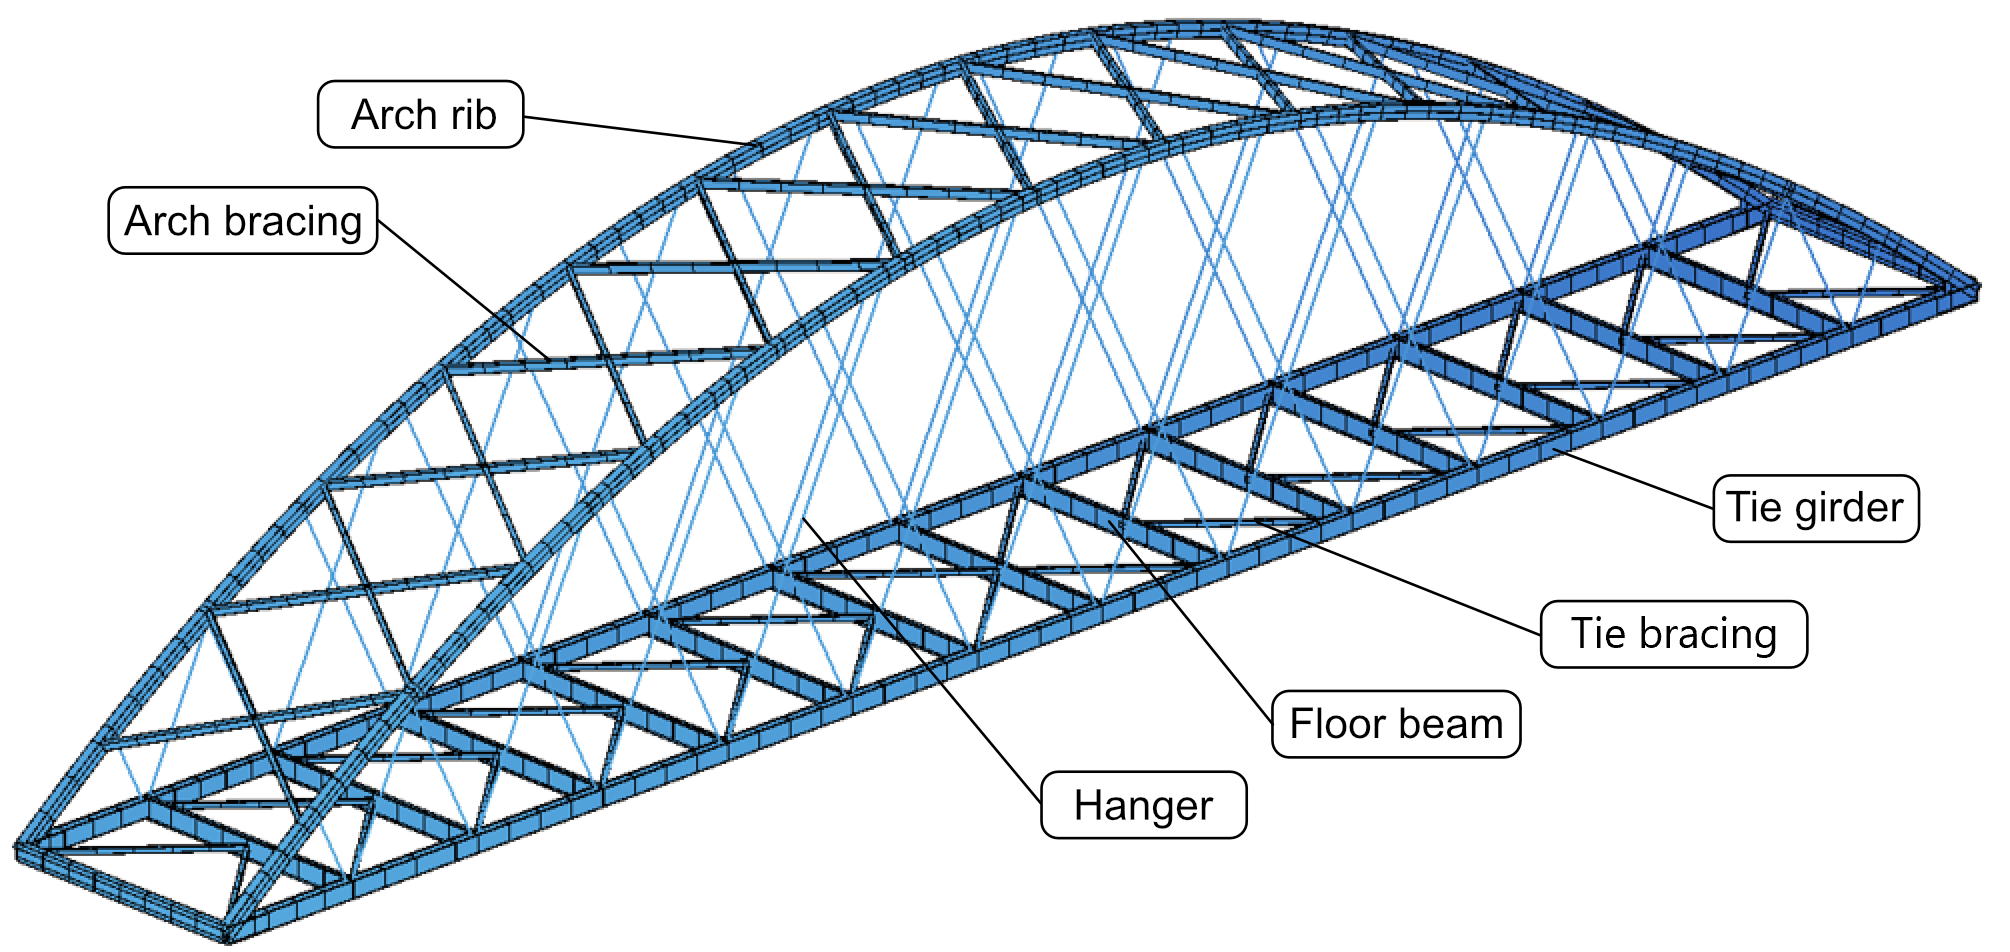
\includegraphics[width=0.8\textwidth]{overleaf/Pictures/illustration_components.PNG}
    \caption{Structural components of a network tied-arch bridge}
    \label{fig:components_illustration}
\end{figure}

The network tied-arch bridge is considered an enhanced construction scheme offering aesthetic appeal and benefits in terms of structural efficiency [cite hu, dai, yan, liu]. Steel bridges of this type require significantly less material and allow for more slender cross-sections compared to other more popular bridge types [cite Herzog]. However, network tied-arch bridges can be considered a complex structural system and the associated challenges are broad and demanding. The design of the hanger arrangement and its initial configuration (self-equilibrium stress state) influence the behaviour under asymmetric live loading, fatigue and cable loss. Many of these challenges have not been addressed satisfactorily [cite Bruno]. Further design variables such as the arch shape and its rise as well as its bracing and inclination have barely been studied. Nevertheless, a strong surge in popularity of this bridge type is observed in the last two decades as can be seen in Fig. [].\\

[Balkendiagramm nach Jahr]\\

The origin of this bridge type can be traced back into the 19th century, when multiple engineers started designing tied-arch bridges featuring a tension chord in the tie. Among these engineers are Joseph Langer and Hermann Lohse who arranged the hangers vertically as shown in Fig. []. In the 1920s, the Danish engineer Octavius F. Nielsen recognised the advantages of inclined hangers, which significantly reduce the longitudinal bending moments and thereby allow for longer spans [cite Nielsen]. Despite showing intersecting hangers in his patent document, he only designed hanger arrangements without intersections [Cite Tveit about network arch]. The structural analysis of a bridge with intersecting hangers was too challenging at the time. Besides that he struggled with hanger loss due to unloading. One of his bridges is presented in Fig. []. \\

[Doppelfigur von Langerscher Balken und Nielsen Brücke]\\

As the live loading increased in the following years the Nielsen-bridges became less suitable. Only by intersecting the hangers, flat hanger inclinations could be obtained, which solve the problem of hanger unloading. The network tied-arch bridge featuring hangers with multiple intersections was introduced by Per Tveit in 1955. The first bridges of this type were built in 1963. One of them, the Fehmarnsundbrücke, which already spanned \SI{248}{m}, is shown in Fig. []. \\

[Fehrmansundbrücke]\\

In the following decades, Per Tveit focused his research on this bridge type, with particular emphasis on the hanger inclination. Despite his efforts, no more bridges of this type were built in Europe until the end of the millennium. However, the idea was exported to Japan, where it became a relevant alternative to classic tied-arch bridges and over 50 bridges of this type were built. In the last two decades, researchers as well as engineers developed more interest in this bridge type, which has now been used around the world. The Blennerhassett Island Bridge (2006), shown in Fig. [], is a particularly large example, which serves as a reference for the investigations in this Thesis.

\subsection{Problem statement} \label{sec:int_prob}
This Master Thesis is part of a series of projects on network tied-arch bridges carried out at the institute of structural engineering at ETH Zurich. A previous Master Thesis carried out by Riccardo Cavegn investigated the optimal arch geometry and the determination of the self-equilibrium stress state. The present thesis aims to gather more insight into structural behaviour with regards to hanger density.
Along with the hanger arrangement, the hanger density is the key parameter determining the fundamental behaviour of this bridge type.\\

\subsection{Definitions} \label{sec:int_def}
\subsubsection{Terminology} 
\subsubsection{Abbreviations}